\section{Auswertung}
  \subsection{Abmessungen und elektrischer Widerstand der Probe}
    Die untersuchte Silberprobe ist $0.022 \si{\milli\meter}$ dick und $14.844 \si{\milli\meter}$ breit sowie
    $25.164\si{\milli\meter}$ lang. Der gemessene elektrische Widerstand beträgt $0.6 \si{\ohm}$.
  \subsection{Untersuchung des Hall-Effektes}
  Im Folgenden sind die Messwerte der Hallspannung tabellarisch dargestellt. $U_{Hall_1}$ bezeichnet dabei die
  gemessene Hallspannung vor der Umpolung und $U_{Hall_2}$ die gemessene Hallspannung nach der Umpolung des
  Magnetfeldes.
    \begin{table}[H]
      \centering
        \caption{Messung der Hall-Spannung mit konstant gehaltenem Probenstrom mit $\SI{5}{\ampere}$.}
        \label{tab:hallspannung1}
        \sisetup{table-format=1.4}
        \begin{tabular}{S S S }
          \toprule
          {$I_{Feld} /\si{\ampere}$} & {$U_{Hall_1} /\si{\milli\volt}$} & {$U_{Hall_2} / \si{\milli\volt}$}\\%, umgepoltes Magnetfeld} \\
          \midrule
          0   & 0.0871 & 0.0031 \\
          0.5 & 0.0885 & 0.0857 \\
          1.0 & 0.0897 & 0.0845 \\
          1.5 & 0.0914 & 0.0829 \\
          2.0 & 0.0926 & 0.0812 \\
          2.5 & 0.0942 & 0.0798 \\
          3.0 & 0.0957 & 0.0785 \\
          3.5 & 0.0971 & 0.0779 \\
          4.0 & 0.0989 & 0.0759 \\
          4.5 & 0.0992 & 0.0748 \\
          5.0 & 0.1002 & 0.0738 \\
          \bottomrule
        \end{tabular}
      \end{table}
      \begin{table}[H]
        \centering
          \caption{Messung der Hall-Spannung mit konstant gehaltenem Spulenstrom mit $\SI{5}{\ampere}$.}
          \label{tab:hallspannung2}
          \sisetup{table-format=1.4}
          \begin{tabular}{S S S }
            \toprule
            {$I_{q} /\si{\ampere}$} & {$U_{Hall_1} /\si{\milli\volt}$} & {$U_{Hall_2} / \si{\milli\volt}$}\\%, umgepoltes Magnetfeld} \\
            \midrule
            0   & 0.0015 & 0.0016 \\
            0.5 & 0.0115 & 0.0088 \\
            1.0 & 0.0213 & 0.0158 \\
            1.5 & 0.0311 & 0.0231 \\
            2.0 & 0.0409 & 0.0300 \\
            2.5 & 0.0507 & 0.0373 \\
            3.0 & 0.0605 & 0.0443 \\
            3.5 & 0.0703 & 0.0513 \\
            4.0 & 0.0802 & 0.0585 \\
            4.5 & 0.0900 & 0.0657 \\
            5.0 & 0.0999 & 0.0727 \\
            \bottomrule
          \end{tabular}
        \end{table}
  \subsection{Berechnung der Leitfähigkeitsparameter}
  Bei den folgenden Rechnungen gibt ein Ergebnis mit Subskript $P$ ein Ergebnis unter Verwendung der Messwerte mit konstantem Platinenstrom und $S$ eines mit
  konstantem Spulenstrom. In den folgenden Berechnungen werden für Physikalische Konstanten der Werte der Scientific
  Python Datenbank verwendet sowie für Unsicherheiten Numeric Python.
    \subsubsection{Anzahl der Ladungsträger pro Volumen}
    \label{sec:ladtrprovol}
        Für die Anzahl der Ladungsträger pro Volumen ergibt sich mit \ref{eqn:Uh2} nach umstellen nach n
        \begin{equation}
            n=-\frac{1}{U_{H} e_0}\frac{B\cdot I_q}{d}. \label{eqn:Uh21}
          \end{equation}
          Dabei bezeichnet $U_{H}$ die Hall-Spannung, $e_{0}$ die Elementarladung, $B$ die magnetische Flussdichte, $I_{q}$ den Platinenstrom und $d$ die Dicke
          der Probe. Mit Gleichung \ref{eqn:Uh21} ergibt sich dann die Anzahl der Ladungsträger pro Volumen für eine Silberprobe zu
          \begin{equation*}
            n_{P} = (-1.0 \pm -0.6) \cdot 10^{28} \frac{1}{\si{\cubic\meter}}
          \end{equation*}
          für konstant gehaltenen Platinenstrom und
          \begin{equation*}
            n_{S} = (-1.7 \pm -1.5) \cdot 10^{28} \frac{1}{\si{\cubic\meter}}
          \end{equation*}
        für konstant gehaltenen Spulenstrom.
        Der Fehler wurde mit Gaußscher Fehlerfortpflanzung
        \begin{equation}
          \sigma_f = \sqrt{\sum_{i=0}^{N} {\frac{\partial f}{\partial x_i} \cdot \sigma_{x_i}}}
          \label{eqn:gauss}
        \end{equation}
        und der Mittelwert durch ein arithmetisches Mittel berechnet. Die Gaußsche Fehlerfortpflanzung und der
        Mittelwert werden im folgenden analog mit Python berechnet.
    \subsubsection{Anzahl der Ladungsträger pro Atom}
      Die Anzahl der Ladungsträger pro Atom berechnet sich mit \ref{eqn:z}.
       Nun ergibt sich für die Anzahl der Ladungsträger pro Atom
       \begin{align*}
         z_{P} & = \frac{n_{P} V_{A}}{N_A} = -0.16 \pm 0.11 \\
         z_{S} & = \frac{n_{S} V_{A}}{N_A} = -0.30 \pm 0.26
       \end{align*}
       Alternativ kann $z$ auch berechnet werden, indem die Masse der Probe durch
       \begin{equation*}
         m_{Probe} = \rho_{Ag} \cdot V_{Probe}
       \end{equation*}
       berechnet wird. Hierbei bezeichnet $\rho_{Ag} = 10490 \si{\kilo\gram\per\cubic\meter}$ die Dichte von Silber und $V_{A}$ das Volumen der Probe.
       Nun wird das Gewicht der Probe durch das Atomgewicht des Silbers geteilt, was die Atomanzahl in der Probe liefert.
       Dann berechnet sich $z$ zu
       \begin{equation*}
         z = \frac{n \cdot V_{A}}{n_{A}}
       \end{equation*}
       wobei $n_{A}$ die Anzahl der Atome in der Probe bezeichnet. Dies liefert diesselben Werte für $z$ wie \ref{eqn:z}.
       bei $20 °C$ und $V_{Probe}$ das Volumen der Silberfolie.
    \subsubsection{Die mittlere Flugzeit}
    \label{sec:mitflugz}
      Die mittlere Flugzeit $\bar{\tau}$ berechnet sich nach
      \begin{equation*}
        \bar{\tau} = \frac{2m_{0}L}{e_{0}^{2}RnQ}
      \end{equation*}
      zu
      \begin{align*}
        \bar{\tau}_{P} & = (-3.4 \pm -2.3) \cdot 10^{-16} \si{\second} \\
        \bar{\tau}_{S} & = (-1.9 \pm -1.7) \cdot 10^{-16} \si{\second}.
      \end{align*}
      Hierbei ist $m_{0} = 9.1122 \cdot 10^{-31} \si{\kilo\gram}$ die Ruhemasse des Elektrons, $L = 25.164 \cdot 10^{-3} \si{\meter}$ die Länge der Probe,
      $e_{0}$ die Elementarladung, $R = 0.6 \si{\ohm}$ der gemessene Widerstand, $n$ die Anzahl der Ladungsträger pro Volumen wie in \ref{sec:ladtrprovol} berechnet
      und $Q = 3.26568 \cdot 10^{-7}$ der Querschnitt der Probe.
    \subsubsection{Die mittlere Driftgeschwindigkeit}
      Die mittlere Driftgeschwindigkeit $\bar{v}_d$ berechnet sich nach \ref{eqn:vd} aus
      \begin{equation}
        \bar{v}_d = \frac{j}{e_{0} \cdot n}.
      \end{equation}
      Hierbei bezeichnet $j = 1 \si{\ampere\per\cubic\milli\meter}$ die Stromdichte und $n$ die Anzahl der Ladungsträger pro Volumen, analog zu \ref{sec:mitflugz}.
      Dann ergibt sich
      \begin{align*}
        \bar{v}_{dP} & = (7 \pm 4) \cdot 10^{-10} \si{\meter\per\second} \\
        \bar{v}_{dS} & = (3.6 \pm 3.2) \cdot 10^{-10} \si{\meter\per\second}
      \end{align*}
    \subsubsection{Die Beweglichkeit}
      Die Beweglichkeit $\mu$ wird nach \ref{eqn:mu} berechnet durch
      \begin{equation}
        \mu = -\frac{e_{0} \cdot \bar{\tau}}{2 \cdot m_{0}}.
      \end{equation}
      $m_{0}$ bezeichnet die Ruhemasse des Elektrons. Mit $\bar{\tau}$ aus Abschnitt \ref{sec:mitflugz} ergibt sich
      \begin{align*}
        \mu_{P} & = (3.0 \pm 2.0) \cdot 10^{-5} \si{\coulomb\second\per\kilo\gram}\\
        \mu_{S} & = (1.7 \pm 1.5) \cdot 10^{-5} \si{\coulomb\second\per\kilo\gram}
      \end{align*}
    \subsubsection{Die Totalgeschwindigkeit}
    \label{sec:totgeschw}
      Um die mittlere Totalgeschwindigkeit zu berechnen, muss zuerst die Fermi-Energie bekannt sein. Diese berechnet sich nach
      \begin{equation}
        E_{F} = \frac{h^{2}}{2m_{0}} \cdot \sqrt[3]{\left(\frac{3n}{8 \pi}\right)^{2}}
      \end{equation}
      wobei $h$ die Planck-Konstante, $m_{0}$ die Ruheenergie des Elektrons und $n$ die Anzahl der Ladungsträger pro Volumen bezeichnet. Damit ergibt sich dann
      \begin{align*}
        E_{FP} & = (2.6 \pm 1.2) \cdot 10^{-19} \si{\joule} \\
        E_{FS} & = (3.9 \pm 2.3) \cdot 10^{-19} \si{\joule}
      \end{align*}
      Die Totalgeschwindigkeit $|v|$ wird berechnet durch
      \begin{equation}
        |v| = \sqrt{\frac{2 \cdot E_{F}}{m_{0}}}.
      \end{equation}
      Einsetzen der Werte für $E_{F}$ und $m_{0}$ ergibt nun
      \begin{align*}
        |v|_{P} & = (7.6 \pm 1.7)\cdot 10^{5} \si{\meter\per\second}\\
        |v|_{S} & = (9.3 \pm 2.7)\cdot 10^{5} \si{\meter\per\second}
      \end{align*}
    \subsubsection{Die mittlere freie Weglänge}
      Die mittlere freie Weglänge $\bar{l}$ berechnet sich mit
      \begin{equation}
        \bar{l} = \bar{\tau} \cdot |v|
      \end{equation}
      Mit den Werten aus Abschnitt \ref{sec:mitflugz} sowie \ref{sec:totgeschw} ergibt sich nun
      \begin{align*}
        \bar{l_{P}} & = (-2.6 \pm 1.1)\cdot 10^{-10}  \si{\meter} \\
        \bar{l_{S}} & = (-1.8 \pm 1.0)\cdot 10^{-10}  \si{\meter}
      \end{align*}
  \subsection{Die magnetische Flussdichte in Abhängigkeit des Feldstroms}
  \begin{table}[H]
    \centering
      \caption{Messung der Magnetischen Flussdichte und des Feldstroms}
      \label{tab:flussdichte1}
      \sisetup{table-format=4.1}
      \begin{tabular}{S S}
        \toprule
        {$I_{Feld} /\si{\ampere}$} & {$B /\si{\milli\tesla}$} \\
        \midrule
        0   &   21.6 \\
        0.5 &  127.8 \\
        1.0 &  247.5 \\
        1.5 &  360.7 \\
        2.0 &  466.0 \\
        2.5 &  565.1 \\
        3.0 &  667.0 \\
        3.5 &  803.0 \\
        4.0 &  949.5 \\
        4.5 & 1082.9 \\
        5.0 & 1154.6 \\
        \bottomrule
      \end{tabular}
    \end{table}
    \begin{table}[H]
      \centering
        \caption{Messung der Magnetischen Flussdichte und des Feldstroms mit umgepoltem Feld}
        \label{tab:flussdichte2}
        \sisetup{table-format=4.1}
        \begin{tabular}{S S}
          \toprule
          {$I_{Feld} /\si{\ampere}$} & {$B /\si{\milli\tesla}$} \\
          \midrule
          0   &   23.8 \\
          0.5 &   94.0 \\
          1.0 &  214.4 \\
          1.5 &  330.0 \\
          2.0 &  445.1 \\
          2.5 &  556.3 \\
          3.0 &  662.1 \\
          3.5 &  767.6 \\
          4.0 &  863.9 \\
          4.5 &  952.6 \\
          5.0 & 1031.9 \\
          \bottomrule
        \end{tabular}
      \end{table}
      Die in den obigen Tabellen \ref{tab:flussdichte1} und \ref{tab:flussdichte2} dargestellten Messwerte werden
      im Folgenden graphisch dargestellt.
      \begin{figure}
        \centering
          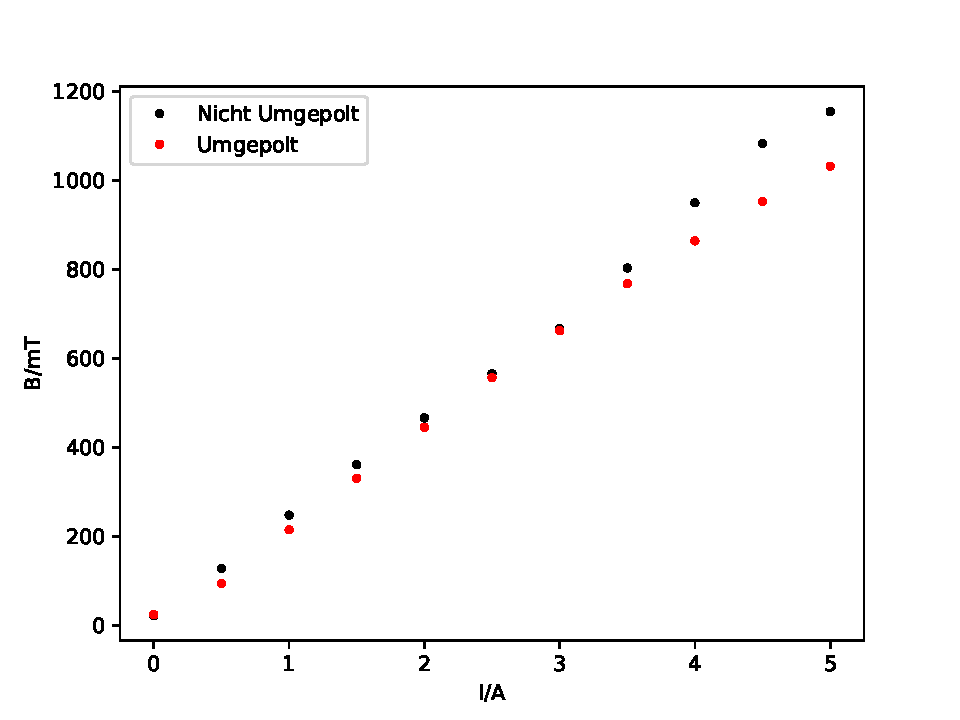
\includegraphics[width=\textwidth]{auswertung/magnetplot1.pdf}
          \caption{Die Messwerte der Magnetischen Flussdichte des Magnetfeldes in Abhängigkeit zum Spulenstrom.}
          \label{fig:magnet1}
      \end{figure}
      Die Messwerte steigen linear mit dem Spuhlenstrom an, man sieht jedoch, dass der Anstieg bei der nicht umgepolten
      Messung ein wenig höher ausfällt als bei der umgepolten Messung.
  \label{sec:Auswertung}
